\chapter{Graphs and data}
\label{ch:graphs}

\chapquote{There is a magic in graphs. The profile of a curve reveals in a flash a whole situation -- the life history of an epidemic, a panic, or an era of prosperity. The curve informs the mind, awakens the imagination, convinces.}{Henry D. Hubbard, US National Bureau of Standards}

In \cref{ch:sequences} we investigated pictures patterns (fractals by Koch and Sierpi\'nski, and patterns made of square tiles) and used those pictures to generate sequences of numbers. We begin this chapter with a discussion of another way to represent our sequences of numbers visually: by making a coordinate graph. Then, we will extend these ideas to create visual representations of other mathematical objects, and of scientific (and other) data.

% % % % % % % % % % % % % % % % % % % % % % % % % % % % % % % % % % % % % % % % 
\section{Coordinate graphing}
\label{sec:coordgraph}

\Cref{fig:coordplane} summarizes the familiar landmarks of the \gls{coordinate plane}. We see the horizontal \gls{x-axis} and the vertical \gls{y-axis}. Using the two axes as number lines, we can locate \glspl{ordered pair} of numbers using the convention $(x,y)$. The points $(7, \umin2)$ and $(\umin6, 3)$ have been plotted as examples. The point $(0,0)$ where the the two axes meet, is a special point called the \gls{origin}.

\begin{figure}
	\centering
	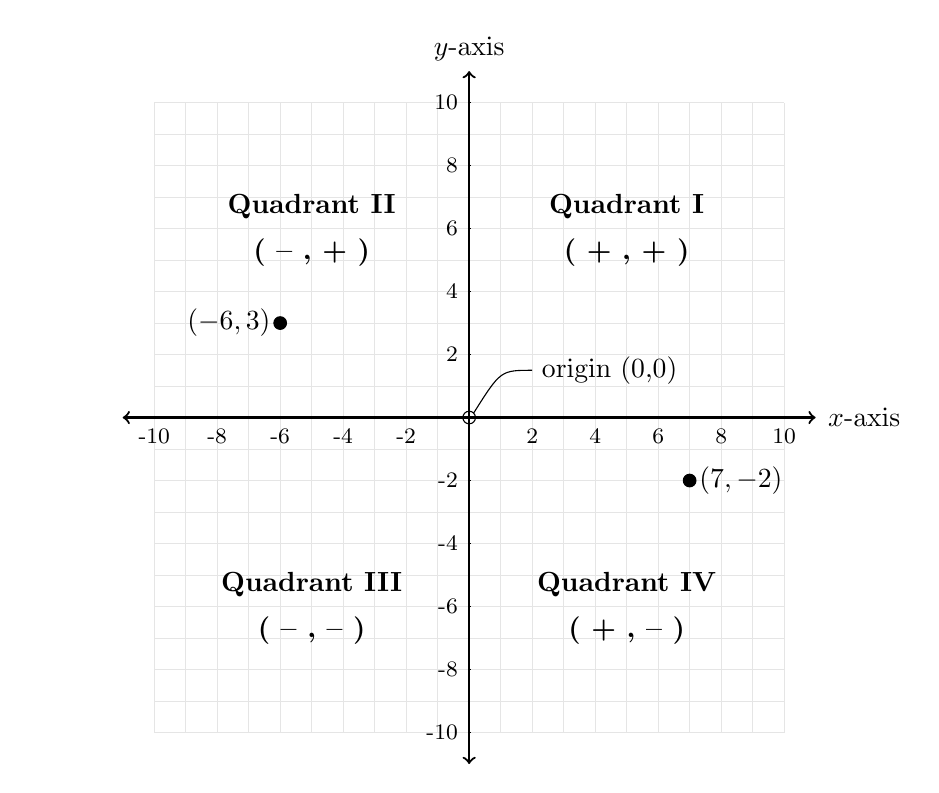
\begin{tikzpicture}[scale=0.4]
		%% grid setup
		\draw[very thin, color=gray!20] (-10,-10) grid (10, 10);
		\draw[<->,thick] (-11,0) -- (11,0);
		\draw (14,0) node[left]{$x$-axis};
		\draw (-14,0) node[right] {};
		\draw[<->,thick] (0,-11) -- (0,11) node[above]{$y$-axis};
		\foreach \x in {-10,-8,...,-2,2,4,...,10}
			\draw (\x,0.05) -- (\x,-0.05) node[below] {\footnotesize\x};
		\foreach \y in {-10,-8,...,-2,2,4,...,10}
			\draw (0.05,\y) -- (-0.05,\y) node[left] {\footnotesize\y};
		%% Quadrants
		\draw (5,6) node[above]{\bfseries Quadrant I}
			node[below]{\bfseries ( + , + 	)};
		\draw (-5,6) node[above]{\bfseries Quadrant II}
			node[below]{\bfseries ( -- , + )};
		\draw (-5,-6) node[above]{\bfseries Quadrant III}
			node[below]{\bfseries ( -- , -- )};
		\draw (5,-6) node[above]{\bfseries Quadrant IV}
			node[below]{\bfseries ( + , -- )};
		%% Origin
		\draw (0,0) circle (0.2);
		\draw (45:0.2) .. controls (1,1.5) .. (2,1.5) node[right]{origin (0,0)};
		%% Sample points
		\draw[fill] (7,-2) circle (0.2) node[right]{$(7, -2)$};
		\draw[fill] (-6,3) circle (0.2) node[left]{$(-6, 3)$};
	\end{tikzpicture}
	\caption{The coordinate plane and its important landmarks}
	\label{fig:coordplane}
\end{figure}

The axes chop the plane into four regions called \glspl{quadrant}, which are numbered starting in the upper right and moving counter-clockwise (as shown in the figure). The signs in parentheses indicate the signs of the $x$- and $y$-coordinates in each quadrant. The $x$-coordinates of the points in Quadrants I and IV are positive, while points in Quadrants II and III have $x$-coordinates that are negative. Points with positive $y$-coordinates lie in Quadrants I and II, while points with negative $y$-coordinates fall in Quadrants III and IV.\footnote{A point that lies on an axis doesn't actually lie in any of the four quadrants. So, the point $(4, 0)$ lives on the positive $x$-axis, but neither in Quadrant I nor in Quadrant IV.}

\begin{boxexplore}[Pizza intersections]
Bob's friend Melvin ``Hambone'' Jones once worked delivering pizzas in his hometown of Euclid, Ohio. The town has streets running north-south and east-west.\footnote{Euclid, Ohio is also the home of the Polka Hall of Fame, though that has nothing to do with this problem. Also, Euclid isn't laid out in a grid as this problem implies, though it should be, given its name.}

Hambone is currently parked at the intersection we will call $(0,0)$. If he drives one block east, he will arrive at the intersection $(1,0)$. If he then turns right and drives one block south, he will arrive at the intersection $(1,-1)$.

Starting from $(0,0)$, describe are all the intersections that Hambone can reach by driving a total distance of exactly 10 blocks.
\end{boxexplore}

\kverse{Melvin ``Hambone'' Jones delivers pizzas in Euclid, Ohio.}

\addtodoitem{Was there any Krumbli stuff in the sequences chapter? We need some continuity...}

\subsection{Graphing a sequence}

Our goal is to make a visual representation of a sequence on the coordinate plane.

``But,'' you may be asking yourself, ``a sequence is just a list of numbers. How do we make a coordinate graph, which needs coordinate pairs of numbers? It takes \textit{two numbers} to make a \textit{pair}!''

To graph a sequence, we use the term number as the $x$-coordinate and the term's value as the $y$-coordinate. Consider the sequence $1, 2, 4, 8, 16, 32,\dotsc$. The first term is 1, the second term is 2, and so on. We can organize this in a table, and write out the ordered pairs. Then, we can plot those ordered pairs and see a visual representation of our sequence!

\resizeplot{0}{0}{7}{40}

\bigskip
\begin{minipage}[c]{0.5\textwidth }
	\centering
	\begin{tabular}{|C{0.25\linewidth}|C{0.25\linewidth}|C{0.25\linewidth}|}
	\hline
	\text{Term No.} & \text{Term Value} & \text{Coord. Pair}\\
	x & y & (x,y)\\\hline
	1 & 1 & (1,1)\\
	2 & 2 & (2,2)\\
	3 & 4 & (3,4)\\
	4 & 8 & (4,8)\\
	5 & 16 & (5,16)\\
	6 & 32 & (6,32)\\\hline
	\end{tabular}
\end{minipage}%
%
\begin{minipage}[c]{0.5\textwidth }
	\centering
	\begin{tikzpicture}
		\begin{axis}[
			fullsize,
			defaultgrid,
			allminorticks,
			labeloutsideaxis,
			xlabel={Term No.},
			ylabel={Term Value},
		]
		\addplot[algpoints, blue] coordinates {(1,1)(2,2)(3,4)(4,8)(5,16)(6,32)};
		\end{axis}
	\end{tikzpicture}
\end{minipage}
\medskip

Recall that that sequence above, where the terms have a constant ratio, is called a geometric sequence. Let's look at an example of an arithmetic sequence, in which the terms have a constant difference. For example, consider the sequence $8, 13, 18, 23, 28, 33,\dotsc$. This sequence produces the following table and graph:

\bigskip
\begin{minipage}[c]{0.5\textwidth }
	\centering
	\begin{tabular}{|C{0.25\linewidth}|C{0.25\linewidth}|C{0.25\linewidth}|}
	\hline
	\text{Term No.} & \text{Term Value} & \text{Coord. Pair}\\
	x & y & (x,y)\\\hline
	1 & 8 & (1,8)\\
	2 & 13 & (2,13)\\
	3 & 18 & (3,18)\\
	4 & 23 & (4,23)\\
	5 & 28 & (5,28)\\
	6 & 33 & (6,33)\\\hline
	\end{tabular}
\end{minipage}%
%
\begin{minipage}[c]{0.5\textwidth }
	\centering
	\begin{tikzpicture}
		\begin{axis}[
			fullsize,
			defaultgrid,
			allminorticks,
			labeloutsideaxis,
			xlabel={Term No.},
			ylabel={Term Value},
		]
		\addplot[algpoints, red] coordinates {(1,8)(2,13)(3,18)(4,23)(5,28)(6,33)};
		\end{axis}
	\end{tikzpicture}
\end{minipage}
\medskip

Finally, let's see what a quadratic pattern looks like. For example, the perfect squares form a quadratic sequence $1, 4, 9, 16, 25, 36, \dotsc$. Their table and graph go like this:

\bigskip
\begin{minipage}[c]{0.5\textwidth }
	\centering
	\begin{tabular}{|C{0.25\linewidth}|C{0.25\linewidth}|C{0.25\linewidth}|}
	\hline
	\text{Term No.} & \text{Term Value} & \text{Coord. Pair}\\
	x & y & (x,y)\\\hline
	1 & 1 & (1,1)\\
	2 & 4 & (2,4)\\
	3 & 9 & (3,9)\\
	4 & 16 & (4,16)\\
	5 & 25 & (5,25)\\
	6 & 36 & (6,36)\\\hline
	\end{tabular}
\end{minipage}
%
\begin{minipage}[c]{0.5\textwidth }
	\centering
	\begin{tikzpicture}
		\begin{axis}[
			fullsize,
			defaultgrid,
			allminorticks,
			labeloutsideaxis,
			xlabel={Term No.},
			ylabel={Term Value},
		]
		\addplot[algpoints, violet] coordinates {(1,1)(2,4)(3,9)(4,16)(5,25)(6,36)};
		\end{axis}
	\end{tikzpicture}
\end{minipage}
\medskip

Take a moment to compare the graphs of these three sequences. How are they alike? How are they different?

\subsection{Features of the graph of a sequence}

Note that since the term number is always greater than 0, our graphs only show the positive part of the $x$-axis. We'll soon see that this is an artificial limitation that doesn't apply to most situations: the negative part of the $x$-axis is just as important as the positive part.

Note also that we haven't connected the dots. A sequence has a first term and a second term, but no one-and-a-halfth term. So, we shouldn't have any points with $x$-coordinates in between the natural numbers. We'll soon see that this is an artificial limitation, too. Fractional $x$-values are appropriate for most rules.

If we change our point of view and allow the input to be any real number, we will have turned our sequence into a mathematical relationship called a \gls{function}.\footnote{Actually, a sequence is \textit{already} a function. The distinction we make here has to do with what kinds of input values are allowed. Later, once we have some additional concepts under our belts, we'll talk about a sequence as ``a function whose domain is the natural numbers''.} We'll discuss the details of what functions are (and what they are not) in \cref{ch:functions}.


% % % % % % % % % % % % % % % % % % % % % % % % % % % % % % % % % % % % % % % % 
\section{Algebraic expressions}
\label{sec:algexpr}

\begin{boxexplore}[Don't take all year]
Find three natural numbers $x$, $y$, and $z$ which satisfy the equation $28x + 30y + 31z = 365$. Can you find more than one set of numbers $x,y,z$ that satisfy the equation?
\end{boxexplore}

In \cref{ch:numbers} we used the order of operations to simplify numeric expressions, which are made up of numbers and arithmetic operators. For example, \[3\cdot4-8(4^2-1)\] is a numeric expression. It contains only numbers and operators and, in the end, it simplifies down to a single number.\footnote{Spoiler alert: It's $-108$.} An \gls{algebraic expression} on the other hand can contain letters in addition to numbers and operators, for example \[3x - 5y + 18.\] These letters, called \glspl{variable}, stand in for numbers that we don't know or which may change.

\begin{boxdef}[Variable]
A representation of a value that can change. In algebra, variables are often represented by letters. We usually use letters from the Latin alphabet ($a, b, c, d,\dotsc$), but we sometimes also use other symbols, such as letters from the Greek alphabet ($\alpha, \beta, \gamma, \delta, \dotsc$).
\end{boxdef}

\begin{boxdef}[Algebraic expression]
A symbolic representation of mathematical operations that can involve both numbers and variables.
\end{boxdef}

\subsection{Numbers and variables}

In your mathematical career so far, you have probably worked with letters that stand in for numbers. Recall the formula for the circumference of a circle: \[C = \pi d.\]
This formula explains the relationship between $d$, which stands in for the diameter of some circle, and $C$, which stands for the circumference of that circle. The letters $d$ and $C$ are variables. They stand in for numbers that can change, depending on which circle we're talking about.\footnote{Note that $\pi$ is \textit{not} a variable. We use a (Greek) letter in this case not because the value of $\pi$ might change, but because it's an irrational number that is impossible to write out in full. We often use letters to stand in for mathematical objects that are inconvenient, sometimes impossible, to write down in another way: $e$, $i$, $\phi$, and $\aleph_0$ each has a special mathematical meaning.}

Once we start to introduce letters into our expressions, we have to discuss some standard notation and terminology. As we have seen, we don't usually write any multiplication symbol when multiplying a number by a variable. Rather than writing $3\cdot x$ or $3(x)$, we can write $3x$ without anything in between.

An algebraic expression that is built using only multiplication (or division) is called a \gls{term}. For example, $3x$ and $\frac{1}{2}m$ are terms. On the other hand, the expression $3x+2y$ is not a term because it includes addition. In fact, this expression is the sum of two terms.

\begin{boxdef}[Term]
An algebraic expression that represents only multiplication and division between variables and constants (numbers).
\end{boxdef}

When we have the product of a number and a variable, like $3x$ or $\umin11g$, the number part is called the \gls{coefficient} of the term. So, the coefficient of $3x$ is 3, and $\umin11$ is the coefficient of $\umin11x$. If we have a variable all alone without a number attached, like $y$ or $w$, then we picture a ``phantom 1'' lurking there as the coefficient: $y$ is the same as $1y$, and $1w$ is the same as $w$.

\begin{boxdef}[Coefficient]
The numerical factor in a term with a variable. If no number is explicitly written, the coefficient is understood to be 1.
\end{boxdef}

\subsection{Evaluating algebraic expressions}

A variable is a ``placeholder'' that stands in for a number. We can only determine the value of an algebraic expression if we know what numbers the different variables represent.

Consider the expression $3x$. If we know that $x$ represents $15$, then we can \gls{evaluate} the expression $3x$ in the case that $x = 15$. In that case, it must be that $3x = 3(15) = 45$.

When we evaluate an algebraic expression, we substitute in values for its variables, and then simplify the resulting numeric expression using the order of operations. It is a really good habit always to use parentheses when substituting numeric values for variables. This can avoid confusion about negative numbers!

\begin{boxex}
\label{ex:evaluating}
Evaluate the expressions (a) $6x+ 4$, and (b) $x^2 - 5$ for the $x$ values 3, $\umin1$, and $\frac{1}{2}$.

\exsoln{}
\begin{enumerate}[label={(\alph*)}]
\item To evaluate the expression $6x + 4$ for the given values of $x$, we simply substitute and follow the order of operations.
\[
\begin{array}{lllll}
\text{When $x=3$:}
&
&
\text{When $x=\umin1$:}
&
&
\text{When $x=\frac{1}{2}$:}
\\ % content
\begin{aligned}
6x + 4 & = 6(3) + 4\\
& = 18 + 4\\
& = 22
\end{aligned}
&
\qquad\qquad
&
\begin{aligned}
6x + 4 & = 6(\umin1) + 4\\
& = \umin6 + 4\\
& = \umin2
\end{aligned}
&
\qquad\qquad
&
\begin{aligned}
6x + 4 & = 6\left(\tfrac{1}{2}\right) + 4\\
& = 3 + 4\\
& = 7
\end{aligned}
\end{array}
\]

\item We do the same in order to evaluate $x^2 - 5$ for the given $x$ values.
\[
\begin{array}{lllll}
\text{When $x=3$:}
&
&
\text{When $x=\umin1$:}
&
&
\text{When $x=\frac{1}{2}$:}
\\ % content
\begin{aligned}
x^2 - 5 & = (3)^2 - 5\\
& = 9 - 5\\
& = 4
\end{aligned}
&
\qquad\qquad
&
\begin{aligned}
x^2 - 5 & = (\umin1)^2 - 5\\
& = 1 - 5\\
& = \umin4
\end{aligned}
&
\qquad\qquad
&
\begin{aligned}
x^2 - 5 & = \left(\tfrac{1}{2}\right)^2 - 5\\
& = \tfrac{1}{4} - 5\\
& = -\tfrac{19}{4}
\end{aligned}
\end{array}
\]
\end{enumerate}
\end{boxex}

Note how the parentheses help out when $x = \umin1$. Without those parentheses, we would have run the risk of making the most common mistake in Algebra 1! Remember the difference between $(\umin1)^2$ and $\umin1^2$.

%%Speaking of parentheses: Remember that a graphing calculator will follow the order of operations. That means that we need to use the proper notation for our intentions. If our intent is to raise $\umin2$ to the fourth power, we had better not write $\umin2^4$ but rather write $(\umin2)^4$ with parentheses!

%%% WHAT TO DO WITH THIS STUFF?
%(2) NO WORK NO CREDIT always applies. If you are wondering how to show work when you have a calculator at your disposal, here is what I want. Be sure to write down what you are having the calculator do for you. Say you need to add 3/4 to 1/2 and then divide it by 7. You need to write down ( 3/4 + 1/2) / 7. That way I know what you are doing to solve the problem.
%
%(3) SIMPLIFY COMPLETELY always applies. Your answers need to be simplified improper fractions, unless the solution is in a context or I ask you specifically for a different format. Be sure to read questions carefully.
%
%(4) A few things we will go over in class over about operating the TI-84+:
%a. what button to use to designate a negative
%b. what to do when you have a syntax error
%c. how to enter fractions and other short-cut keys
%d. how to raise to powers other than 2 e. how to clear ram
%f. how to correct the mode/setting
%g. how to recall, delete, and insert
%h. how to simplify answers
%
%We will go over more things your calculator can do for you as they become necessary in class.

% MOVE TO FUNCTIONS CHAPTER...?
%Using the formula for the formula for arithmetic, I wrote the rule an = 12 + 3 (n – 1), which I convert to the equation y = 12 + 3 (x – 1). Now let's graph it in a standard window. You should be able to see why they call this relationship linear. Arithmetic sequences always graph to be lines, not vertical or horizontal though. Arithmetic sequences always increase or decrease by the exact same value, which means they have a constant rate of change.

% % % % % % % % % % % % % % % % % % % % % % % % % % % % % % % % % % % % % % % % 
\section{Graphing a function}
\label{sec:graphingfunc}

The graphs of sequences that we created earlier were quite limited. Since sequences use only the natural numbers as input values, the only points we had available to plot were the points where $x = 1, 2, 3, 4, \dotsc$. But now, knowing how to evaluate algebraic expressions, we can create more complete graphs by choosing a wider variety of $x$-values.

\begin{boxexplore}[Extending our sequences]
Write a zero-based explicit rule for the arithmetic sequence shown below (this is the second example from \cref{sec:coordgraph}). First write the rule in terms of $n$ and $a_n$, then translate your rules into a graphable format in terms of $x$ and $y$.
\[8, 13, 18, 23, 28, \dotsc\]
The given sequence represents the $y$-values of the rule for the $x$-values 1, 2, 3, 4, and 5. Evaluate your rule for the $x$-values 0, -1, -2, -3, -4, and -5. Then, plot these 11 points on a coordinate grid.
\end{boxexplore}

The rule for the sequence in the startup exploration is $a_n = 5n + 3$, or in terms of $x$ and $y$, we have the rule $y = 5x + 3$. To create the coordinate graph, we can substitute the different $x$-values into the rule and compute the $y$-values. The middle column in the table below is our ``process column'' in which we substitute an $x$-value and compute the corresponding $y$-value. 

\begin{table}
\begin{tabular}{|C{2cm}|C{6cm}|C{2cm}|}
	\hline
	x & y = 5 x + 3& (x,y)\\\hline
	0 		& y = 5(0) + 3 = 0 + 3 = 3 & (0,3)\\
	\umin1 & y = 5(\umin1) + 3 = \umin5 + 3 = \umin2  & (\umin1,\umin2)\\
	\umin2 & y = 5(\umin2) + 3 = \umin10 + 3 = \umin7  & (\umin2,\umin7)\\
	\umin3 & y = 5(\umin3) + 3 = \umin15 + 3 = \umin12  & (\umin3,\umin12)\\
	\umin4 & y = 5(\umin4) + 3 = \umin20 + 3 = \umin17  & (\umin4,\umin17)\\
	\umin5 & y = 5(\umin5) + 3 = \umin25 + 3 = \umin22  & (\umin5,\umin22)\\\hline
\end{tabular}
\end{table}

In the end, we generate 6 new coordinate pairs, which we can graph alongside the five points that we were given.

\resizeplot{-5}{-25}{5}{29}
\begin{center}
\begin{tikzpicture}
	\begin{axis}[
		medsize,
		defaultgrid
	]
	\addplot[algpoints, red] coordinates {(-5,-22)(-4,-17)(-3,-12)(-2,-7)(-1,-2)(0,3)(1,8)(2,13)(3,18)(4,23)(5,28)};
	\end{axis}
\end{tikzpicture}
\end{center}

Can you anticipate the location of the point that we plot when $x = \frac{1}{3}$? What about when $x = \umin\frac{5}{2}$? What would our graph look like if we used all of the points in $\R$ as the $x$-values?

When we use all of the real numbers as input to the rule $y = 5x + 3$, the resulting graph is a straight line. Of course, it would be impossible to actually plot \textit{all} of the points (there are infinitely many of them), but the pattern holds true, and so we can replace the dots with a continuous line.

\begin{center}
\begin{tikzpicture}
	\begin{axis}[
		medsize,
		defaultgrid
	]
	\addplot[algcurve, red, domain=-5:5] (\x,5*\x+3);
	\end{axis}
\end{tikzpicture}
\end{center}

The rules below correspond to the other two sequences we studied in \cref{sec:coordgraph}. Under each rule is the graph that is created when we plot the rule over $\R$.

\begin{figure}
\begin{minipage}[c]{0.49\textwidth }
	\centering
	$y = 2^x$\par\medskip
	\begin{tikzpicture}
		\begin{axis}[
			fullsize,
			defaultgrid
		]
		\addplot[algcurve, blue, domain=-5:4.75] (\x,2^\x);
		\end{axis}
	\end{tikzpicture}
\end{minipage}
%
\begin{minipage}[c]{0.49\textwidth }
	\centering
	$y = x^2$\par\medskip
	\begin{tikzpicture}
		\begin{axis}[
			fullsize,
			defaultgrid
		]
		\addplot[algcurve, violet, domain=-5:5] (\x,\x^2);
		\end{axis}
	\end{tikzpicture}
\end{minipage}
\end{figure}

Are you surprised by these two graphs? Back in \cref{sec:coordgraph}, the graphs of these two sequence looked similar. But, we were only looking at the first quadrant! Their graphs are very different for negative values of $x$.

The moral of the story is that when we are asked to graph an equation by hand, we need to use a variety of different $x$-values, including negative numbers and fractions. Often, a problem will clearly indicate exactly what values to use.

\subsection{Criteria for high quality graphs}

In algebra we make a distinction between ``sketching'' and ``graphing''. A sketch is just a quick drawing and it doesn't need to be super accurate. A sketch can drawn on notebook paper (or scribbled on a napkin).

On the other hand, a proper graph is meant to communicate something to the viewer. A graph must be accurately drawn on graph paper. The most important features of whatever we're graphing -- a sequence, a function, a plot of a data set -- must be clear, accurate, and neatly represented. Here are some guidelines for creating high-quality graphs.

High quality graphs should be drawn on graph paper. An individual graph does not have to take up an entire piece of graph paper, although it should be drawn large enough to be easily understood.

Use a ruler or straightedge to make straight lines, in particular the coordinate axes or any linear data. Plus, we should draw arrowheads on anything that continues forever. This includes axes, lines, and curves (note the arrowheads in the graphs above).

Be mindful when choosing a scale for the axes. Choose a scale that fits the data and ensures that your graph shows all important features of the curve. The origin does not necessarily need to be in the center of the grid. For example, if we are plotting data that includes only positive values, then we only need the first quadrant. The origin in this case might be in the lower left-hand corner of the graph.

Scales for the $x$- and $y$-axes can be different, and in some cases must be different, so this can take a little bit of planning. The scale must be the same for the whole length of an axis, and cannot have any ``jumps'' or ``breaks''. Changes in the scale will distort the shape of the graph, which defeats the purpose! Compare the two grids below. The grid on the left is fine, but the grid on the right includes a common mistake. Can you identify the problem?

\begin{minipage}{0.5\linewidth}
	\centering
	OK!\par
	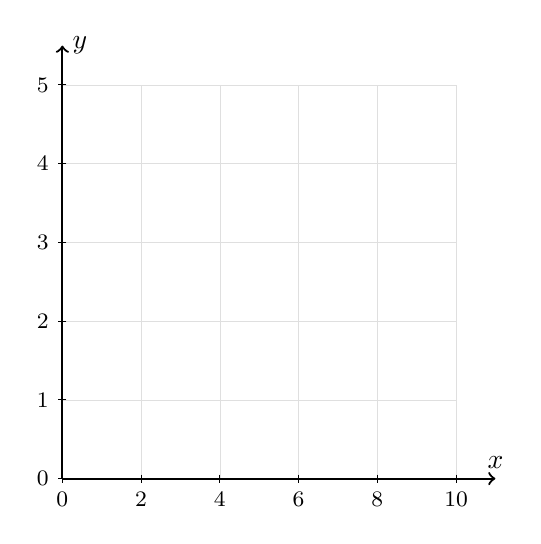
\begin{tikzpicture}[scale=1]
		%% grid setup
		\draw[very thin, color=gray!25] (0,0) grid (5,5);
		\draw[->,thick] (0,0) -- (5.5,0) node[above]{$x$};
		\draw[->,thick] (0,0) -- (0,5.5) node[right]{$y$};
		\foreach \x in {0,2,...,10}
			\draw (\x/2,0.05) -- (\x/2,-0.05) node[below] {\footnotesize\x};
		\foreach \y in {0,1,...,5}
			\draw (0.05,\y) -- (-0.05,\y) node[left] {\footnotesize\y};
	\end{tikzpicture}
\end{minipage}
%
\begin{minipage}{0.5\linewidth}
	\centering
	Not OK!\par
	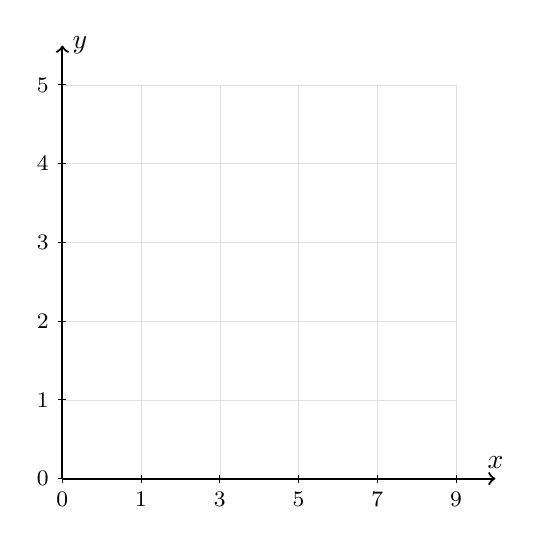
\begin{tikzpicture}[scale=1]
		%% grid setup
		\draw[very thin, color=gray!25] (0,0) grid (5,5);
		\draw[->,thick] (0,0) -- (5.5,0) node[above]{$x$};
		\draw[->,thick] (0,0) -- (0,5.5) node[right]{$y$};
		\foreach \x in {0,1}
			\draw (\x,0.05) -- (\x,-0.05) node[below] {\footnotesize\x};
		\draw (2,0.05) -- (2,-0.05) node[below] {\footnotesize3};
		\draw (3,0.05) -- (3,-0.05) node[below] {\footnotesize5};
		\draw (4,0.05) -- (4,-0.05) node[below] {\footnotesize7};
		\draw (5,0.05) -- (5,-0.05) node[below] {\footnotesize9};
		\foreach \y in {0,1,...,5}
			\draw (0.05,\y) -- (-0.05,\y) node[left] {\footnotesize\y};
	\end{tikzpicture}
\end{minipage}
\medskip

High quality graphs are clearly labeled. The scale should be indicated on the axes, and the axes should be labeled. For graphs of equations, this might mean simply labeling the axes $x$ and $y$. When plotting data, include more informative names like ``time'' or ``distance''.

A final question to consider regarding data points: to connect or not to connect? In the next section, we will discuss this question in some detail. But we've already seen some important pieces of this puzzle. When we have a sequence, or other data that skips values, we should not connect the points.

If we do want to connect the points, say, when graphing a funcction by plotting some sample points, we should connect with a smooth curve and \textit{not} individual line segments. If we use a straight line to connect points, then we are telling our audience that the data in between the points is linear, which may not be the case! Go back and have a look at the graph of $y=x^2$. It doesn't come to a point at the bottom. Rather it's a smooth curve that passes through the origin.

%\begin{boxexplore}[Extended exploration: Big graphs]
%\addtodoitem{Click here to visit the extended exploration: Big Graphs}
%\end{boxexplore}
\addtodoitem{Link to extended exploration: Big graphs}

% % % % % % % % % % % % % % % % % % % % % % % % % % % % % % % % % % % % % % % % 
\section{Patterns in data}
\label{sec:patternsindata}

The graphs that we have been working with so far have been very orderly. Technical and scientific data, however, are not always so tidy. Data can be noisy, messy, and incomplete. We will need some tools that can help us to see and describe patterns that may (or may not) exist in experimental data.

%\begin{boxexplore}[Extended exploration: Who is the best age guesser?]
%\addtodoitem{Click here to visit the extended exploration: Who Is the Best Age Guesser?}
%\end{boxexplore}
\addtodoitem{Link to extended exploration: Age guesser}

\begin{boxexplore}[Water consumption]
The graph shown in \cref{fig:waterconsumption} depicts water consumption in Edmonton, capital of the Canadian province of Alberta, during the gold medal men's ice hockey game at the 2010 Winter Olympics in Vancouver. The game was played between Canada and United States.

Water consumption during the game is shown in blue, while data from the same time period on the previous day is shown in green.

Write down anything you notice or wonder about the data presented in this graph.

A few notes: Ice hockey games are played in three 20-minute periods with breaks in between. In this particular game, the score was tied at the end of regular play. Canada scored the winning goal in overtime and was then awarded the gold medal.
\end{boxexplore}

\begin{figure}[htbp]
\centering\bigskip
\begin{tikzpicture}
\begin{axis}[
		width=0.75\textwidth,
		ylabel={\footnotesize Customer Water Demand (megaliters)},
		ymin=300,
		ymax=500,
		ytick={320,340,...,480},
		ytick pos=left,
		ymajorgrids,
		xmin=0,
		xmax=6,
		xtick={0,...,6},
%		xtick pos=left,
		xticklabels={12:00, 13:00, 14:00, 15:00, 16:00, 17:00, 18:00},
		tick label style={
			font=\footnotesize
		},
		legend style={
			font=\footnotesize,
			legend pos=north west,
			draw=black!25
		},
		enlargelimits=false
	]
	\addplot[thick, green!80!black] table [x=time, y=day1, col sep=comma] {data/water.csv};
	\addlegendentry{27 Feb 2010};
	\addplot[thick, blue] table [x=time, y=day2, col sep=comma] {data/water.csv};
	\addlegendentry{28 Feb 2010};
\end{axis}
\end{tikzpicture}
\caption{Water consumption in Edmonton on 27 and 28 February 2010 (source: \href{http://www.epcor.com}{EPCOR})}
\label{fig:waterconsumption}
\end{figure}

%\begin{figure}[!htbp]
%	\centering
%	{\color{black!25}\fbox{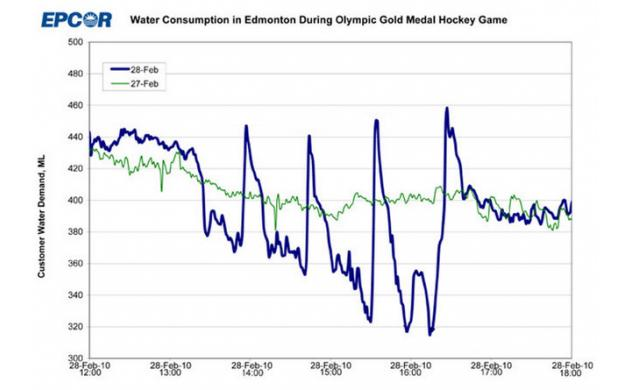
\includegraphics[scale=0.65]{canadianwater.png}}}
%	\caption{Water consumption in Edmonton during the 2010 Olympic men's ice hockey final}
%	\label{fig:waterhockey}
%\end{figure}

%\begin{boxexplore}[Guess Your Weight]
%\begin{minipage}[t]{0.7\textwidth}
%\vspace{0pt}
%Alphonse the Amazing has a Guess-Your-Weight booth on the carnival midway at the Cheeseville Zoo. To play, people pay \$1, Alphonse guesses their weight, and then they step on a scale (only the most self-confident people play this game). If Alphonse's guess is off by more than 5 pounds (over or under), they win a prize.
%
%The table shows the guessed weight and actual weight of 15 brave souls who played the game.
%
%Evaluate Alphonse's skill as a weight guesser, based on the evidence presented in the table. What feedback would you give him?
%\end{minipage}%
%%
%\begin{minipage}[t]{0.3\textwidth}
%\vspace{0pt}
%\raggedleft
%\begin{tabular}{|C{1.55cm}|C{1.55cm}|}
%\hline
%\text{\footnotesize Guessed Wt} & \text{\footnotesize Actual Wt}
%\\\hline
%75 & 71\\
%90 & 88\\
%100 & 99\\
%130 & 121\\
%140 & 126\\
%175 & 159\\
%95 & 93\\
%115 & 112\\
%125 & 118\\
%150 & 134\\
%80 & 78\\
%160 & 145\\
%180 & 163\\
%85 & 82\\
%170 & 153\\\hline
%\end{tabular}\par
%\end{minipage}
%\end{boxexplore}

In the graph of Edmonton water consumption, the amount of water being used varies depending on the time of day (not the other way around). We say that ``time of day'' is the \textit{independent variable} and ``water demand'' is the \textit{dependent variable}. 

\begin{boxdef}[Independent variable]
A variable whose values affect the values of another variable. In a graph of the relationship between two variables, the quantity represented on the horizontal axis (the $x$-axis) usually represents the independent variable.
\end{boxdef}

\begin{boxdef}[Dependent variable]
A variable whose values depend on the values of another variable. In a graph of the relationship between two variables, the quantity represented on the vertical axis (the $y$-axis) usually represents the dependent variable.
\end{boxdef}

\subsection{Correlation}

We can compare just about any two quantities. One way to do this is with a graph called a \gls{scatter plot}.

\begin{boxdef}[Scatter plot]
A graph that relates data of two different sets. The two sets of data are displayed as ordered pairs.
\end{boxdef}

Suppose we wish to compare, say, the height and weight for all of the players on the top two 2010 Olympic men's ice hockey teams. Let's make a graph comparing every player's height and weight as ordered pairs: (height, weight). This graph is shown on the left in \cref{fig:hockeystats}.\footnote{Data from the International Olympic Committee, as reported in \href{http://en.wikipedia.org/wiki/Ice_hockey_at_the_2010_Winter_Olympics}{Wikipedia}.}

While we're at it, let's make another comparison. The graph on the right in \cref{fig:hockeystats} plots every player's height and jersey number as ordered pairs (height, jersey number). What do you notice about these two graphs? How are they the same? How are they different?

\begin{figure}
\label{fig:hockeystats}
\caption{Comparing the Canadian and US men's ice hockey teams (2010 Winter Olympics).}
%
\begin{minipage}{0.45\linewidth}
% (height, weight)
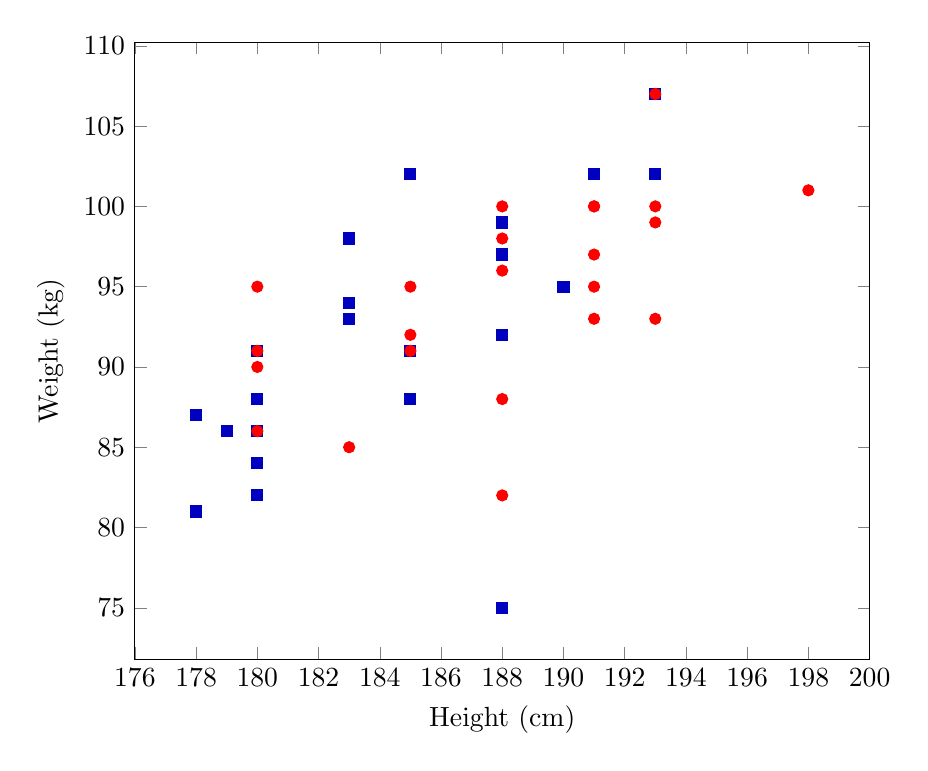
\begin{tikzpicture}[domain=150:200]
	\begin{axis}[
		legend style={
			font=\footnotesize,%
			legend pos=south east,%
			legend cell align=left,%
			/tikz/every even column/.append style={column sep=1em},%
			draw=black!25,%
		},%
		legend columns=-1,
		legend to name=namedhockeylegend,
		width=0.9\linewidth,%
		xlabel={Height (cm)},%
		ylabel={Weight (kg)}%
	]
	\addplot[%
		scatter/classes={
			1={mark=square*, blue!75!black},%
			2={mark=*, red}
		},
		scatter,
		only marks,
		scatter src=explicit symbolic]
      table[x=x, y=y, meta=label] {
	x		y		label
	188		75		1
	185		91		1
	180		91		1
	183		98		1
	193		107		1
	185		102		1
	188		99		1
	178		87		1
	185		88		1
	190		95		1
	191		102		1
	183		94		1
	180		84		1
	179		86		1
	178		81		1
	188		92		1
	180		82		1
	185		91		1
	193		102		1
	180		86		1
	180		88		1
	188		97		1
	183		93		1
	188		98		2
	188		82		2
	191		93		2
	180		86		2
	185		92		2
	183		85		2
	185		91		2
	198		101		2
	191		100		2
	191		97		2
	188		88		2
	180		90		2
	193		100		2
	191		100		2
	185		95		2
	188		100		2
	180		95		2
	193		99		2
	180		91		2
	191		95		2
	193		93		2
	193		107		2
	188		96		2
	};
	\legend{Team USA, Team Canada};
	\end{axis}
\end{tikzpicture}
\end{minipage}
%
\begin{minipage}{0.45\linewidth}
% (height, jersey number)
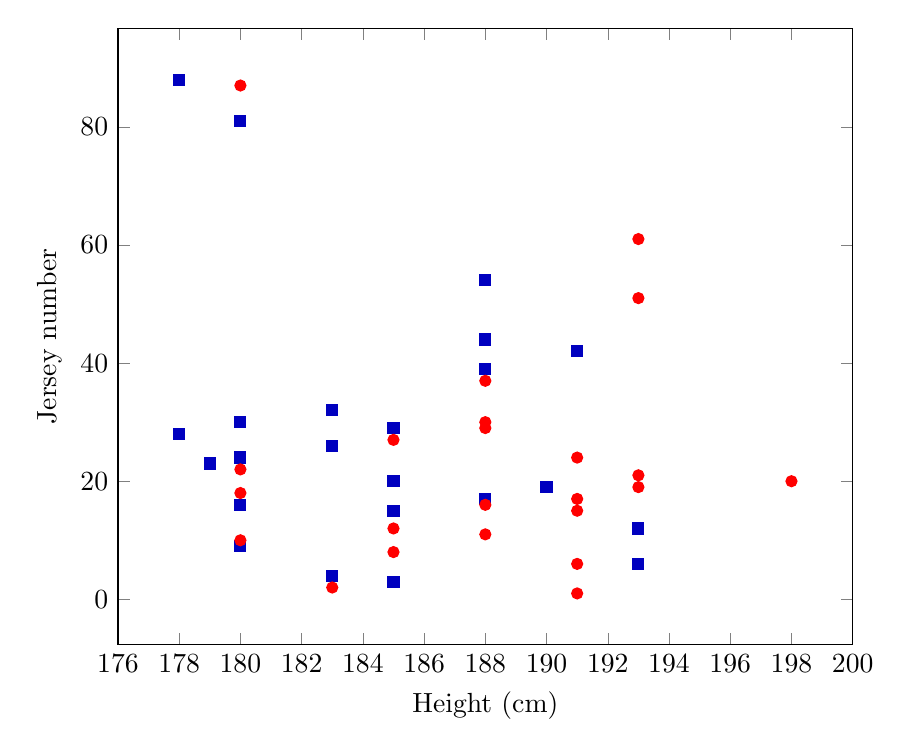
\begin{tikzpicture}[domain=150:200]
	\begin{axis}[
		width=0.9\linewidth,%
		xlabel={Height (cm)},%
		ylabel={Jersey number}%
	]
	\addplot[%
		scatter/classes={
			1={mark=square*, blue!75!black},%
			2={mark=*, red}
		},
		scatter,
		only marks,
		scatter src=explicit symbolic]
      table[x=x, y=y, meta=label] {
	x		y		label
	188		39		1
	185		29		1
	180		30		1
	183		4		1
	193		6		1
	185		3		1
	188		44		1
	178		28		1
	185		20		1
	190		19		1
	191		42		1
	183		32		1
	180		24		1
	179		23		1
	178		88		1
	188		17		1
	180		81		1
	185		15		1
	193		12		1
	180		9		1
	180		16		1
	188		54		1
	183		26		1	
	188		30		2
	188		29		2
	191		1		2
	180		22		2
	185		8		2
	183		2		2
	185		27		2
	198		20		2
	191		17		2
	191		6		2
	188		37		2
	180		87		2
	193		51		2
	191		15		2
	185		12		2
	188		11		2
	180		10		2
	193		61		2
	180		18		2
	191		24		2
	193		21		2
	193		19		2
	188		16		2
	};
	%\legend{Team USA, Team Canada};
	\end{axis}
\end{tikzpicture}
\end{minipage}
\ref{namedhockeylegend}
\end{figure}

Notice that the graph of weight and height has a clear upward slant. This seems reasonable: the taller someone is, the more we might expect that person to weigh. There are some data points that don't fit the trend, but generally speaking the data points are increasing as we look toward the right on the graph. We say that this data shows a positive \gls{correlation}.

\begin{boxdef}[Correlation]
A trend between two sets of data, as seen in a scatter plot. A trend can show positive, negative, or no correlation. Positive correlation shows an \gls{increasing} trend in data. Negative correlation shows a \gls{decreasing} trend in data.
\end{boxdef}

The graph of jersey number versus height is more of a blob. There's no clear trend in this data, and so we say that is shows \textit{no correlation}. This makes sense, too: there's no logical connection between a player's height and the number they wear on their shirt.

A third possibility would be data which shows a negative correlation, meaning that the data are decreasing as we look towards the right on the graph. Can you imagine two variables that might show a negative correlation when compared on a scatter plot?

Graphing experimental data on a scatter plot helps us to see if there is a relationship between variables. If there is, a pattern will emerge in the graph. The points will fall (approximately) in a line or a curve and will have a correlation. A key thing to remember when it comes to looking at data is that ``correlation does not imply causation''. In other words: If we see that two variables are correlated, we might be tempted to assume that the change in one variable \textit{causes} the change in the other. This is sometimes true, but not always.

%If the scatter plot shows a positive correction, it means that as the independent variable increases, the dependent variable increases. If the scatter plot shows a negative correlation, it means that as the independent variable increases, the dependent variable decreases. If a scatter plot shows no correlation, it indicates that there is no relationship between the two variables.

For example, it seems reasonable to believe that a change in height will cause a change in weight. But, there is data that shows a positive correlation between ``consumption of mozzarella cheese per person'' and ``number of civil engineering doctorates awarded''. This has to be a coincidence! There's no (good) reason to think that changing one of these variables would cause a change in the other one.\footnote{This fact is courtesy of the website \href{http://www.tylervigen.com/view_correlation?id=3890}{Spurious Correlations}, which has many graphs of interesting and ridiculous data that show correlation but not causation. Sometimes, it's fun to try to ``explain'' the correlation. Perhaps in this case the increase in mozzarella cheese consumption is due to an increase in takeout pizza demand, which leads to more pizza delivery shops, which in turn requires more roads, which means we need more engineers to design them.}

\subsection{Continuous and discrete data}

When we drew the graph of a sequence, we didn't connect the dots. A sequence has a first term and a second term, but no one-and-a-halfth term. The $x$-values have no ``in-betweens''.

Similarly, imagine a graph showing ``time'' as the independent variable and ``number of hockey players on the ice'' as the dependent variable. In this case, the $y$-values would have no ''in-betweens''. There could be 11 players or 12 players on the ice, but never 11.5 players. This is called \gls{discrete data}.

\begin{boxdef}[Discrete data]
Data for which it doesn't make sense for measurements to exist between given data points. Discrete data often involves \textit{counting items}, such at the number of cars in a parking lot over time. 
\end{boxdef}

On the other hand, when we started to picture the graph of a rule that could accept any real number as input, we drew a continuous line on the graph. The graph of water consumption in Edmonton, is jagged, spiky, and irregular -- but it's a continuous line. We can measure how much water has been used at any point in time, and we can measure the amount of water in fractions of a unit. We call this \gls{continuous data}.

\begin{boxdef}[Continuous data]
Data that has no holes, gaps, or breaks. Continuous data often involves \textit{measuring some value} where measurements exist (and may change) between data points. For example, a person's height over time.
\end{boxdef}

%The graphs we saw in the last section (straight lines and smooth curves) are quite easy to describe mathematically. For instance, we know how to write rules for sequences, and sequences were what led us to graph those curves in the first place. It's hard -- and sometimes impossible -- to write a neat rule for this data. So, we have developed some other terminology to describe sometimes-messy data.

%The key to knowing the difference between continuous and discrete data is to ask whether the data involves measuring or counting.

\kverse{We consider graphs showing ``Bob's distance from home'', and ``number of customers in line at the Middle Market cheese counter''.}

Consider a data collection scenario in which we want to graph ``Bob's distance from home at any given time (in kilometers)''. Bob is always a certain distance away from home (perhaps 0 km, if he is at home), and he could be any distance (even fractions of a kilometer). So, this is continuous data and our graph should be an unbroken line.

Now consider the scenario in which we graph ``number of customers in line at the cheese counter at Middle Market.'' Although there is always a certain number of people in line (maybe zero), there can never be 5.7 people in line. We must count people, and so this data is discrete. Our graph would have to ``jump'' from 5 people to 6 people without going through the in-between values.

\resizeplot{0}{0}{7}{7}
\begin{figure}
\label{fig:continuousvsdiscrete}
\caption{Comparing graphs of continuous and discrete data.}
\begin{minipage}{0.48\textwidth}
\centering
Continuous data\par\medskip
\begin{tikzpicture}
	\begin{axis}[
		fullsize,
		defaultgrid,
		allminorticks,
		labeloutsideaxis,
		xlabel={Time},
		ylabel={Dist. from home (miles)}
	]
	\addplot[samples=400, ultra thick, blue, domain=0.05:6.55]%
		 (\x, -0.12*x^4+1.51*x^3-6.05*x^2+8.64*x-0.38);
	\end{axis}
\end{tikzpicture}
\end{minipage}
%%
\begin{minipage}{0.48\textwidth}
\centering
Discrete data\par\medskip
\begin{tikzpicture}
	\begin{axis}[
		fullsize,
		defaultgrid,
		allminorticks,
		labeloutsideaxis,
		xlabel={Time},
		ylabel={No. customers}
	]
	\draw[line width=2.5pt, blue] (axis cs: 0,1) -- (axis cs: 2,1);
	\draw[line width=2.5pt, blue] (axis cs: 2,2) -- (axis cs: 3,2);
	\draw[line width=2.5pt, blue] (axis cs: 3,6) -- (axis cs: 5,6);
	\draw[line width=2.5pt, blue] (axis cs: 5,5) -- (axis cs: 6,5);
	\draw[line width=2.5pt, blue] (axis cs: 6,4) -- (axis cs: 7,4);
	\end{axis}
\end{tikzpicture}
\end{minipage}
\end{figure}



% % % % % % % % % % % % % % % % % % % % % % % % % % % % % % % % % % % % % % % % 
\section{Interpreting graphs}
\label{sec:interpgraphs}

In this section, our goal is to hone our skills at understanding what a graph is \textit{communicating}.

%\begin{boxexplore}[Extended exploration: Interpreting graphs with distance match]
%\addtodoitem{Click here to visit the extended exploration: Interpreting Graphs with Distance Match}
%\end{boxexplore}
\addtodoitem{Link to extended exploration: distance match}

\begin{boxexplore}[Yeardleigh's submersible]
Always questing after the most delicious ingredients, Yeardleigh buys an underwater submersible vehicle so that she can hunt the ocean floor for interesting sea plants. The graph below shows the depth of Yeardleigh's submersible over time.

Study the graph. What can you tell about what's happening? Write a short paragraph telling, in words, the same story that the graph is telling visually.

\begin{center}
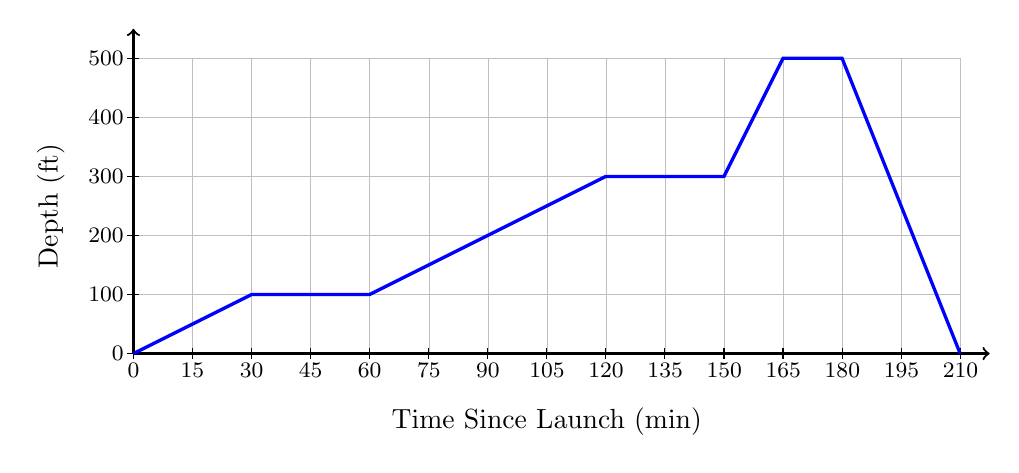
\begin{tikzpicture}[scale=0.75]
	\draw[ultra thin, gray!50] (0,0) grid (14,5);
	\draw[->,thick] (0,0) -- (14.5,0);
	\draw[->,thick] (0,0) -- (0,5.5);
	%% x-axis
	\foreach \x in {0,...,14}
		\draw (\x,0.1) -- (\x,-0.1);
	\foreach \x in {0,15,...,210}
		\draw (0.0667*\x, 0) node[below] {\footnotesize\x};
	\draw (7, -0.75) node[below] {Time Since Launch (min)};
	%% y-axis
	\foreach \y in {0,...,5}
		\draw (-0.1,\y) -- (0.1,\y);
	\foreach \y in {0,100,...,500}
		\draw (0, 0.01*\y) node[left] {\footnotesize\y};
	\draw (-1, 2.5) node[rotate=90,above] {Depth (ft)};
	%% graph
	\draw[very thick, blue] (0,0) -- (2,1) -- (4,1) -- (8,3) -- (10,3) -- (11,5) -- (12,5) -- (14,0);
\end{tikzpicture}
\end{center}
\end{boxexplore}

\kverse{Yeardleigh uses submersible to find new flavors on the ocean floor.}

At the beginning of the trip, Yeardleigh's submersible dives a total of 100 feet in the first 30 minutes. At the end of the trip, it returns to the surface, rising 500 feet in the last 30 minutes. This tells us that the depth of the submersible was \textit{changing much faster} at the end of the journey compared to the beginning.

Note that the graph reflects this: the line is quite steep at the end of the trip and not so steep at the beginning. The steeper the line, the faster the dependent variable is changing with respect to the independent variable.\footnote{We call this the ``rate of change'', and it will become an important focus of our work in \cref{ch:linear}.}

Plus, we can tell from the graph when the submersible is getting deeper (the depth is increasing; the line shows a positive trend) and when it is getting shallower (the depth is decreasing over time; the line shows a negative trend).

Notice that other parts of the graph are horizontal, for example between 30 and 60 minutes. This tells us that the depth of the submersible stayed the same during that time. Of course Yeardleigh could still be moving around below the surface, but she remains at a constant depth, neither diving nor surfacing.

\subsection{Interpreting curves}

Straight lines are fine, but what if the graph shows curved lines? Consider this graph showing the submersible's depth over time. What story would we tell about this graph?

%\resizeplot{0}{0}{100}{500}
%\begin{figure}
%\begin{tikzpicture}
%	\begin{axis}[
%		medsize,
%		defaultgrid,
%		labeloutsideaxis,
%		xlabel={Time (min)},
%		ylabel={Depth (ft)},
%	]
%	\addplot[samples=400, ultra thick, blue, domain=0:100](\x, -0.2*x^2+20*x);
%	\end{axis}
%\end{tikzpicture}
%\end{figure}

\begin{center} %{figure}
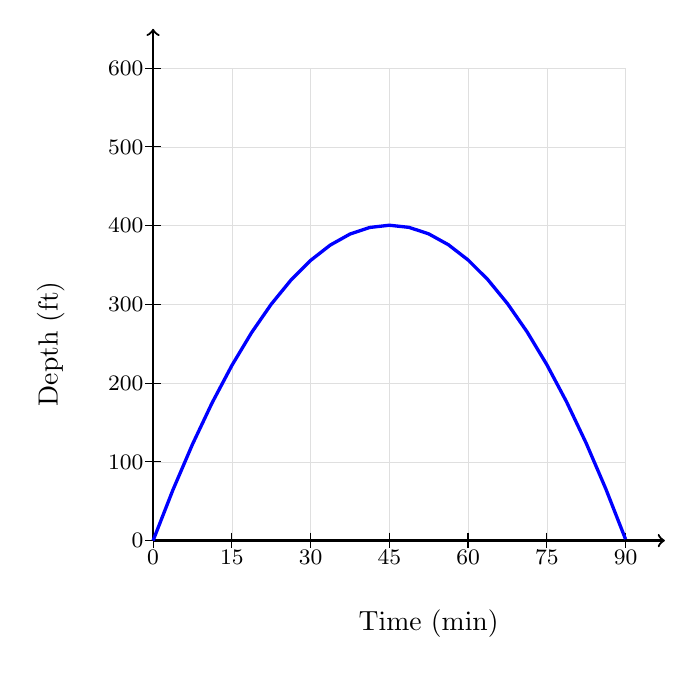
\begin{tikzpicture}[scale=1]
	\draw[ultra thin, gray!25] (0,0) grid (6,6);
	\draw[->,thick] (0,0) -- (6.5,0);
	\draw[->,thick] (0,0) -- (0,6.5);
	%% x-axis
	\foreach \x in {0,...,6}
		\draw (\x,0.1) -- (\x,-0.1);
	\foreach \x in {0,15,...,90}
		\draw (0.0667*\x, 0) node[below] {\footnotesize\x};
	\draw (3.5, -0.75) node[below] {Time (min)};
	%% y-axis
	\foreach \y in {0,...,6}
		\draw (0.1,\y) -- (-0.1,\y);
	\foreach \y in {0,100,...,600}
		\draw (0, 0.01*\y) node[left] {\footnotesize\y};
	\draw (-1, 2.5) node[rotate=90,above] {Depth (ft)};
	%% graph
	\draw[very thick, blue, domain=0:6] plot (\x,-0.444*\x*\x+2.667*\x);
\end{tikzpicture}
\end{center} %{figure}

One way to get a feel for what's happening is to imagine leaning a ruler or pencil against the rounded edge of a soda can. Then picture the ruler rolling along the side of the can, and how the angle of the ruler will change as it rolls.

\begin{figure}
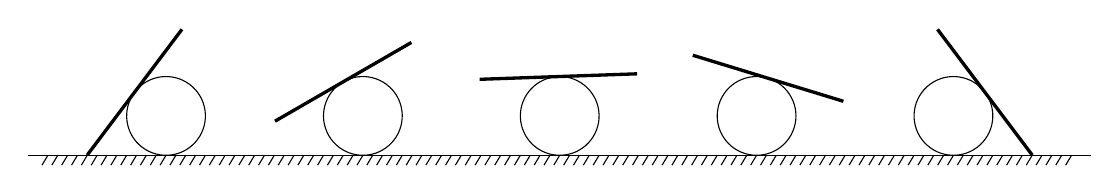
\begin{tikzpicture}[scale=0.5]
	\draw (-1.5,0) -- (25.5,0);
	\foreach \x in {-1,-0.75,...,25} \draw (\x,0) -- (\x-0.15, -0.25);
	\begin{scope}[rotate around={53:(2,1)}]
		\draw (2,1) circle[radius=1cm];
		\draw[very thick] (0,2) -- (4,2);
	\end{scope}
	\begin{scope}[xshift = 5cm, rotate around={30:(2,1)}]
		\draw (2,1) circle[radius=1cm];
		\draw[very thick] (0,2) -- (4,2);
	\end{scope}
	\begin{scope}[xshift = 10cm, rotate around={2:(2,1)}]
		\draw (2,1) circle[radius=1cm];
		\draw[very thick] (0,2) -- (4,2);
	\end{scope}
	\begin{scope}[xshift = 15cm, rotate around={-17:(2,1)}]
		\draw (2,1) circle[radius=1cm];
		\draw[very thick] (0,2) -- (4,2);
	\end{scope}
	\begin{scope}[xshift = 20cm, rotate around={-53:(2,1)}]
		\draw (2,1) circle[radius=1cm];
		\draw[very thick] (0,2) -- (4,2);
	\end{scope}
\end{tikzpicture}
\caption{Pencil rolling along the side of a can}
\end{figure}

Now picture a straight line rolling along the surface of the curved line in the graph above. The straight line approximates the curved line at the point where they touch.

\begin{center} %{figure}
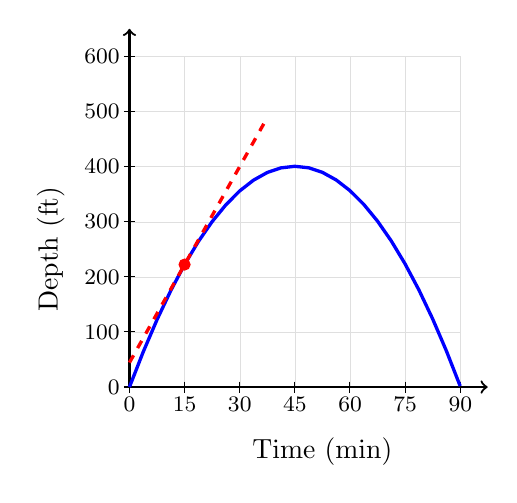
\begin{tikzpicture}[scale=0.7]
	\draw[ultra thin, gray!25] (0,0) grid (6,6);
	\draw[->,thick] (0,0) -- (6.5,0);
	\draw[->,thick] (0,0) -- (0,6.5);
	%% x-axis
	\foreach \x in {0,...,6}
		\draw (\x,0.1) -- (\x,-0.1);
	\foreach \x in {0,15,...,90}
		\draw (0.0667*\x, 0) node[below] {\footnotesize\x};
	\draw (3.5, -0.75) node[below] {Time (min)};
	%% y-axis
	\foreach \y in {0,...,6}
		\draw (-0.1,\y) -- (0.1,\y);
	\foreach \y in {0,100,...,600}
		\draw (0, 0.01*\y) node[left] {\footnotesize\y};
	\draw (-1, 2.5) node[rotate=90,above] {Depth (ft)};
	%% graph
	\draw[very thick, blue, domain=0:6] plot (\x,-0.444*\x*\x+2.667*\x);
	\draw[very thick, dashed, red, domain=0:2.5] plot (\x,1.778*\x+0.444);
	\draw[red,fill=red] (1,2.222) circle[radius=0.1];
\end{tikzpicture}
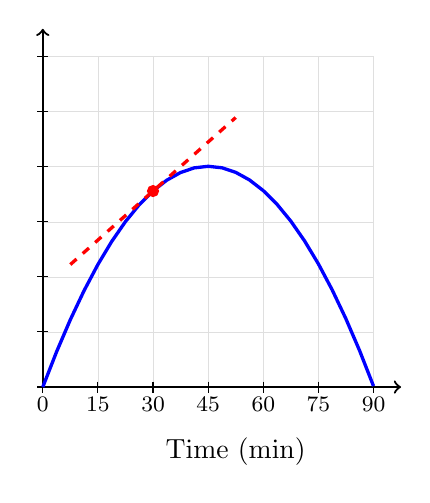
\begin{tikzpicture}[scale=0.7]
	\draw[ultra thin, gray!25] (0,0) grid (6,6);
	\draw[->,thick] (0,0) -- (6.5,0);
	\draw[->,thick] (0,0) -- (0,6.5);
	%% x-axis
	\foreach \x in {0,...,6}
		\draw (\x,0.1) -- (\x,-0.1);
	\foreach \x in {0,15,...,90}
		\draw (0.0667*\x, 0) node[below] {\footnotesize\x};
	\draw (3.5, -0.75) node[below] {Time (min)};
	%% y-axis
	\foreach \y in {0,...,6}
		\draw (-0.1,\y) -- (0.1,\y);
	%\foreach \y in {0,100,...,500}
	%	\draw (0, 0.01*\y) node[left] {\footnotesize\y};
	%\draw (-1, 2.5) node[rotate=90,above] {Depth (ft)};
	%% graph
	\draw[very thick, blue, domain=0:6] plot (\x,-0.444*\x*\x+2.667*\x);
	\draw[very thick, dashed, red, domain=0.5:3.5] plot (\x,0.889*\x+1.778);
	\draw[red,fill=red] (2,3.556) circle[radius=0.1];
\end{tikzpicture}
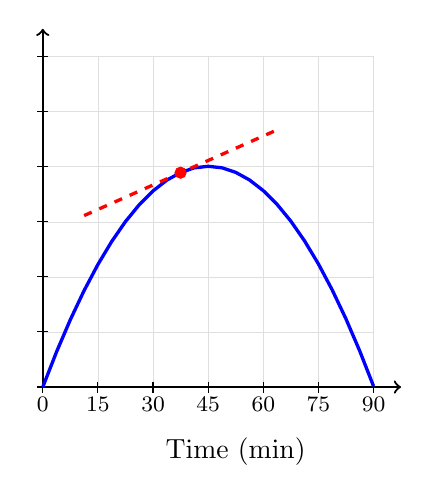
\begin{tikzpicture}[scale=0.7]
	\draw[ultra thin, gray!25] (0,0) grid (6,6);
	\draw[->,thick] (0,0) -- (6.5,0);
	\draw[->,thick] (0,0) -- (0,6.5);
	%% x-axis
	\foreach \x in {0,...,6}
		\draw (\x,0.1) -- (\x,-0.1);
	\foreach \x in {0,15,...,90}
		\draw (0.0667*\x, 0) node[below] {\footnotesize\x};
	\draw (3.5, -0.75) node[below] {Time (min)};
	%% y-axis
	\foreach \y in {0,...,6}
		\draw (-0.1,\y) -- (0.1,\y);
	%\foreach \y in {0,100,...,500}
	%	\draw (0, 0.01*\y) node[left] {\footnotesize\y};
	%\draw (-1, 2.5) node[rotate=90,above] {Depth (ft)};
	%% graph
	\draw[very thick, blue, domain=0:6] plot (\x,-0.444*\x*\x+2.667*\x);
	\draw[very thick, dashed, red, domain=0.75:4.25] plot (\x,0.444*\x+2.778);
	\draw[red,fill=red] (2.5,3.889) circle[radius=0.1];
\end{tikzpicture}
\end{center} %{figure}

We can see that the submersible starts out diving at a fairly high rate. It gradually slows its rate of descent until it eventually stops diving. Then it gradually accelerates as it returns to the surface.\footnote{Believe it or not, this idea -- approximating a curved line with a straight line -- is one of the fundamental motivating ideas in calculus. As you work to interpret these curved graphs, you're growing your calculus brain, right here in Algebra 1. How cool is that?}

\subsection{Impossible situations}

Consider this graph showing the submersible's depth over time. What's going on here?

\begin{center} %{figure}
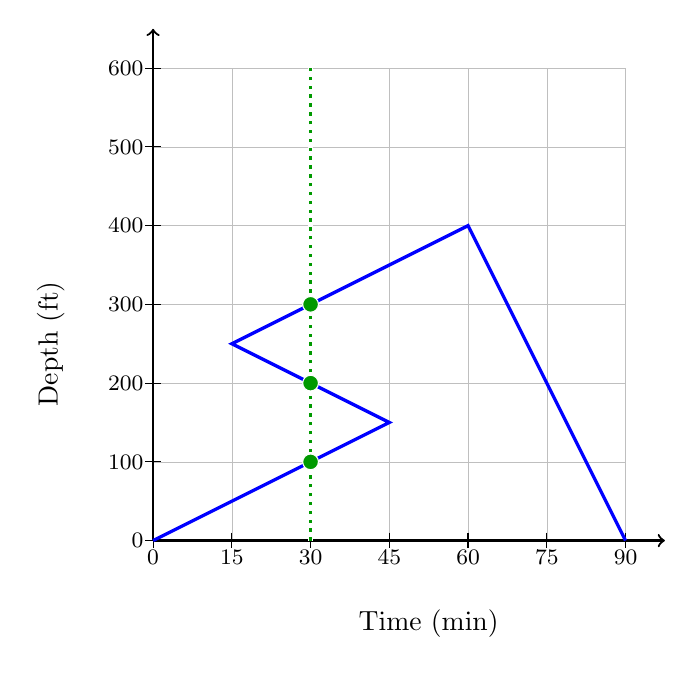
\begin{tikzpicture}[scale=1]
	\draw[ultra thin, gray!50] (0,0) grid (6,6);
	\draw[->,thick] (0,0) -- (6.5,0);
	\draw[->,thick] (0,0) -- (0,6.5);
	%% x-axis
	\foreach \x in {0,...,6}
		\draw (\x,0.1) -- (\x,-0.1);
	\foreach \x in {0,15,...,90}
		\draw (0.0667*\x, 0) node[below] {\footnotesize\x};
	\draw (3.5, -0.75) node[below] {Time (min)};
	%% y-axis
	\foreach \y in {0,...,6}
		\draw (-0.1,\y) -- (0.1,\y);
	\foreach \y in {0,100,...,600}
		\draw (0, 0.01*\y) node[left] {\footnotesize\y};
	\draw (-1, 2.5) node[rotate=90,above] {Depth (ft)};
	%% graph
	\draw[very thick, blue] (0,0) -- (3,1.5) -- (1,2.5) -- (4,4) -- (6,0);
	\draw[ultra thick, white] (2,0) -- (2,6);
	\draw[very thick, dotted, green!60!black] (2,0) -- (2,6);
	\draw[white,fill=green!60!black] (2,1) circle[radius=0.1];
	\draw[white,fill=green!60!black] (2,2) circle[radius=0.1];
	\draw[white,fill=green!60!black] (2,3) circle[radius=0.1];
\end{tikzpicture}
\end{center} %{figure}

This graph is a problem, given the context of ``depth of the submersible over time''. Consider this question: How deep is the submersible 30 minutes after launch?

According to the graph, the submersible is 100 feet deep\ldots\ and 200 feet deep\ldots\ \textit{and} 300 feet deep\ldots\ all at the same time! That's impossible!

This kind of problem could pop up in other places. For example, in a distance-time graph, points that line up vertically mean that something is in more than one place at one instant in time. Though we might wish reality were different, nothing can be in two (or more) places at the same time.

Graphs like this -- where several $y$-values stack up vertically over the same $x$-value -- violate a certain requirement that we will learn about in the next chapter, as we delve into the important mathematical idea of a \textit{function}.

% % % % % % % % % % % % % % % % % % % % % % % % % % % % % % % % % % % % % % % % 
\chaptersummary

In this chapter we began with plotting points to create the graph of a sequence. Then, we built upon these ideas to create the graph of function. We then turned our attention from making graphs to understanding graphs that are given to us.

These two skills -- creating a graph from a given rule, and extracting information from a given graph -- are both key mathematical skills that we will develop in this course. At the heart of both skills lies the connection between a function's rule and its graph. This connection, and more about the concept of a function, are discussed in the next chapter. Onward!

\chaptercopyright
